\documentclass{article}
\usepackage[slovene]{babel}
\usepackage[utf8]{inputenc}
\usepackage[T1]{fontenc}
\usepackage{lmodern}
\usepackage{hyperref}
\usepackage{amsmath}
\usepackage{amsthm}
\usepackage{enumitem}
\usepackage{amssymb}
\usepackage{graphicx}
\usepackage{float}


\newtheorem{definition}{Definicija}[section] 
\newtheorem{theorem1}{Trditev}[section]
\newtheorem{lemma}{Lema}[section]

\title{Projektna naloga iz statistike}
\author{Martin Žust}
\date{2. 1. 2024}

\begin{document}

\section{Analiza prebivalcev mesta Kibergrad}

\subsection{Dohodki po četrtih}
V naši projektni nalogi nas je najprej zanimalo, kako se razlikujejo dohodki družin po četrtih. Opaziti smo želeli ali katera iz med četrti 
posebno izstopa v eno ali drugo smer. S tem namenom smo vzeli enaostavni slučajni vzorec velikosti 100 iz vsake četrti. V isti koordinatni sistem smo nato 
narisali škatlo z brki za vse štiri vzorce, kar je prikazano na sliki \ref{fig:slika1}.

\begin{figure}[H]
    \caption{Dohodki po četrtih}
    \centering
    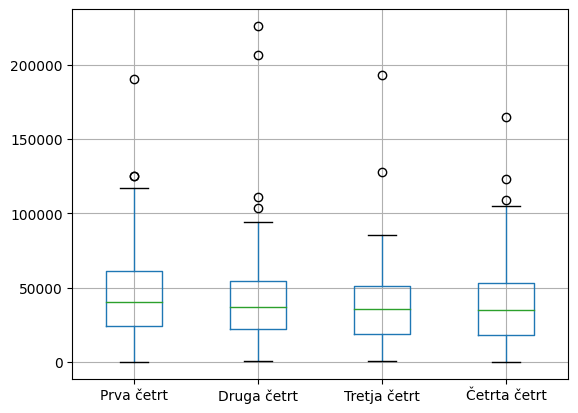
\includegraphics[scale=0.8]{dohodki_po_cetrtih.png}
    \label{fig:slika1}
\end{figure}

Iz slike \ref{fig:slika1} opazimo konkretne razlike med posameznimi četrtmi. Vendar bi lahko prišlo do napake zaradi premajhnih vzorcev. Po limitnih 
zakonih iz teorije verjetnosti namreč vemo, da večji vzorci dajejo večjo gotovost glede reprezentativnosti vzorca glede na celotno populacijo. S tem namenom 
vzamemo še štiri dodatne enostavne slučajne vzorce iz prve (severne) četrti enake velikosti kot prej. Škatle z brki za vseh pet izbranih slučajnih vzorcev iz severne 
četrti je prikazano na sliki \ref{fig:slika2}.

\begin{figure}[H]
    \caption{Slučajni vzorci v prvi četrti}
    \centering
    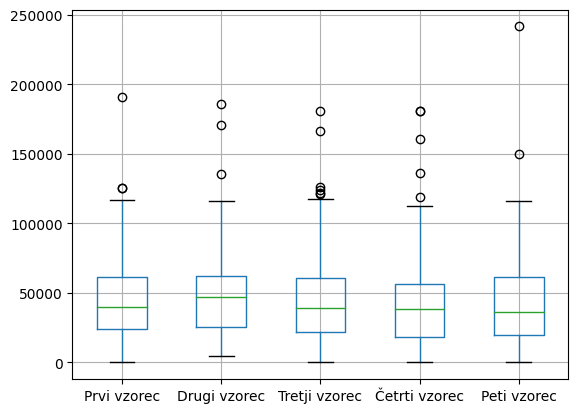
\includegraphics[scale=0.8]{vzorci_severne_cetrti.png}
    \label{fig:slika2}
\end{figure}

Opazimo, da se škatle z brki v prvi četrti med sabo ne razlikujejo nič manj kot škatle z brki po posameznih četrtih. Zaključimo, da so vzorci, ki 
smo jih vzeli premajhni, da bi iz njih lahko potegnili smiselne zaključke. 

%Dodaj vzorce velikosti 2000. 

%Dodaj primerjavo varianc. 

\subsection{Indeks srečnosti}

Za prebivalce mesta Kibergrad definiramo indeks srečnosti družine. Srečnost družine je linearno odvisna od števila otrok, ki jih imajo. Poleg tega vpliv 
izobrazbe na srečnost sledi gostoti normalne porazdelitve. 

\end{document}